\section{Introduction}
to first understand the problem at hand and look at how to proceed, a literature survey was undertaken by us. We scoured through multiple scientific journals and used them as markers for our work. Due to the relative similarity of this problem to that faced in photonics/optics, many papers from an Electrical/Quantum Mechanical background were found. A few papers that developed theory rigorously were also looked at. Below, we shall list out the most important papers in our survey and also explain what each paper contributed to this project. Post that, we describe the approach we plan to take to tackle the problem at hand.


\section{Paper Review}

The first paper is from 1971, from an old soviet journal \cite{zarem} This paper develops the theory from first principles and attempts to solve it using relatively older numerical techniques. This paper clearly explains non-linear phenomena in solid. This paper formed the base of our future work, and our first simulation solver was based on the ideas given in this paper. The paper, besides the rigorous mathematical treatment of the subject at hand, also delves into phonon interaction in materials in brief.

With this background, we derive that there are only a few modes of mixing that is accepted in a material, and these criteria converge whichever approach you take to treat the subject. With a basic phonon treatment of the subject matter, the nuances of wave mixing are also discussed. This is very important and acts as the base on which the rest of the project is built.

This paper was implemented initially, and the results were quite accurate, but this didn't quite serve the purpose of what we set out to do and thus we switched our starting point.

%Put table of Wave Mixing and possible modes and shit. Diagrams also

\begin{figure}
\begin{center}
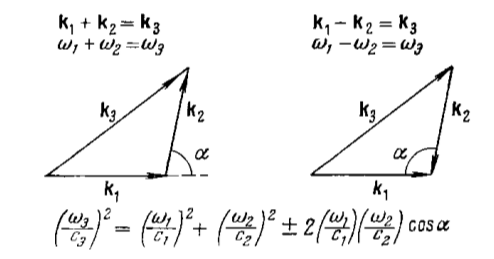
\includegraphics[scale=0.5]
{images/chapter_2/directions_noncollinear.png}
\caption{Direction of resultant wave\cite{zarem}}
\end{center}
\end{figure}

\begin{figure}
\begin{center}
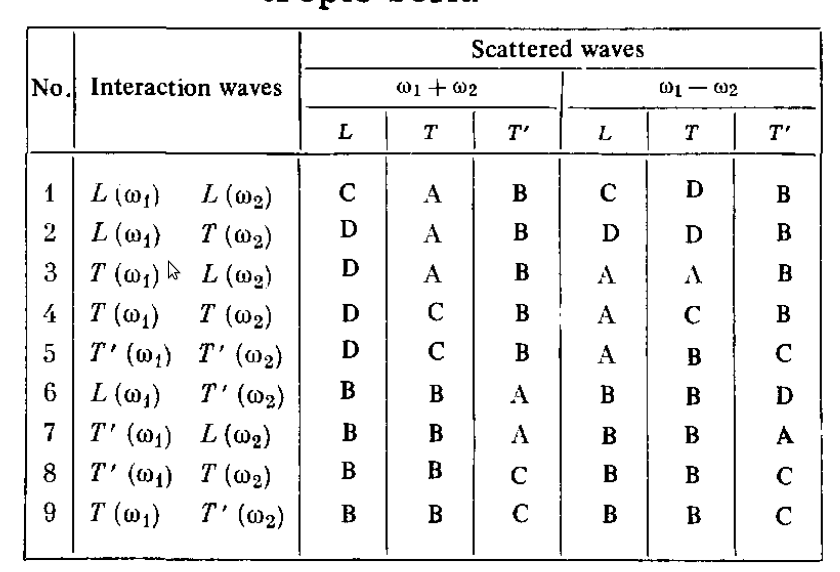
\includegraphics[scale=0.5]
{images/chapter_2/interaction.png}
\caption{Forbidden Modes of Wave Mixing \cite{zarem}}
\end{center}
\end{figure}

The second paper that was pursued post this was a paper on three phonon interaction and a quantum(light) analogue applied to solid material. This paper further expounded on acceptable modes of mixing and also the direction and wave-characteristics of the resulting wave. However, the approach taken by the authors in the paper seemed far too advanced for our purposes and thus this paper was used for experimental setup than the starting point for our work.


The third paper of great significance was that by Liu \cite{Liu}. This paper had a very classical treatment of the governing equation and its solution in a 2 Dimensional collinear environment. The paper was not too advanced and proved useful as our starting point in the simulations. 

The differential equations derived are in two dimensions and could be solved easily. an FDTD method approach was taken over any other approach due to the flexibility of FDTD methods. This paper formed the basis of the forward model and sensitivity analysis. Based on this and a few other readings, we decided to take this approach to tackle the problem.

\begin{figure}
\begin{center}
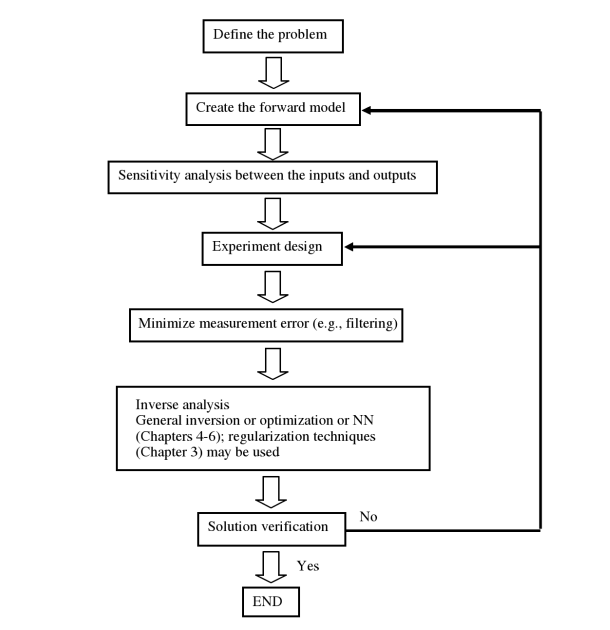
\includegraphics[scale=1]
{images/chapter_2/mthodology_generic.png}
\caption{Generic Methodology of this Project}
\end{center}
\end{figure}

For the inverse model, most of the literature was read from Bishop \cite{bishop} and a few other PhD thesis. This marks the end of literature survey and implementation details of the project